\documentclass{report}





\usepackage[utf8]{inputenc}
\usepackage[T1]{fontenc}
\usepackage[portuguese]{babel}
\usepackage{setspace}
\usepackage{url} 
\usepackage{graphicx} 
\usepackage{hyperref}
\usepackage{amsmath}
\usepackage{ragged2e}
\usepackage{graphicx,color}
\usepackage{natbib}
\usepackage{tocbibind}
\usepackage{indentfirst}
\usepackage{parskip}

 

\title{Trabalho Prático 04 Laboratório de Informática \textbf{\textit {LaTeX}}  \\ \normalsize \singlespacing Relatório desenvolvido sobre o trabalho prático da disciplina de Matemática Discreta}
\author{Victor Destefani \and Pedro Vieira}
\date{\today}

\begin{document}
\maketitle

\begin{abstract} 
\justifying

 No âmbito da disciplina \textbf{Laboratórios de Informática}, foi-nos solicitado a elaboração de um relatório sobre a plataforma \textit{LaTeX}. Contudo, a nossa opção foi selecionar o trabalho prático realizado na disciplina \textbf{Matemática Discreta} para a progressão do mesmo. Buscaremos abordar todos os tópicos que estavam presentes em nosso relatório e expor no novo relatório, efetuando às alterações necessárias de acordo com o que foi solicitado. Todas as questões respondidas a este trabalho, são relativas ao tema das teorias dos grafos. Iremos abordar teoremas como o de Euler, Hamilton, Ore e Dirac com suas sucessivas regras para identificação dos grafos. Também falaremos sobre matriz de adjacência, fecho transitivo e fecho transitivo inverso.
\end{abstract} 

\newpage
\listoffigures
\newpage
\listoftables

\chapter{Introdução}  

Este trabalho foi desenvolvido no âmbito da disciplina de Matemática Discreta, lecionada no curso de Licenciatura em Engenharia de Sistemas Informáticos, do Instituto Politécnico do Cávado e do Ave, presidida pelo Professor Ricardo Gonçalves, com o intuito de aplicar os conhecimentos adquiridos ao longo das sessões sobre a Teoria de Grafos. Para a primeira alínea do trabalho, selecionou-se o mapa de rotas e aeroportos cedidos pela\textbf{Wizz Air Hungary Ltd}, através do website \textbf{https://wizzair.com/pt-pt/voos/mapa}. Para se prosseguir, escolheu-se um aeroporto por país/cidade, que estabelece ponte aérea com Madrid, sendo este o ponto de origem na seleção. Igualmente, houve a inclusão do aeroporto da cidade do Porto, optando somente pelos países/cidades já existentes com a conexão a Madrid. \citet{costa_2018}

\begin{figure}[h]
    \centering
    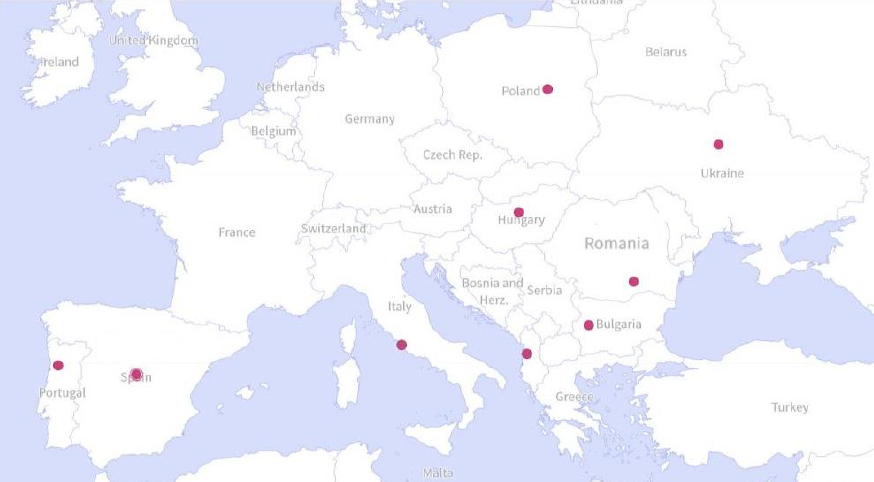
\includegraphics[width=12cm]{Imagem_1_Geral.png}
    \caption{Mapa com as cidades escolhidas.}
    \label{fig1}
\end{figure}

\newpage
\chapter{Questões}
\begin{itemize}
\item 1. Represente a situação escolhida por meio de um grafo.
\item 2. Indique, justificando, se o grafo é conexo.
No contexto do problema, interprete a sua resposta.
\item 3. Indique, justificando, se o grafo é euleriano.
No contexto do problema, interprete a sua resposta.
\item4. Indique, justificando, se o grafo é hamiltoniano.
No contexto do problema, interprete a sua resposta.
\item 5. Apresente a matriz de adjacência do grafo considerado na questão 1.
\item 6. Indique o fecho transitivo direto de um vértice à sua escolha.
No contexto do problema, apresente uma interpretação para o conjunto obtido.
\item 7. Indique o fecho transitivo inverso de um vértice à sua escolha.
No contexto do problema, apresente uma interpretação para o conjunto obtido.
\end{itemize}

\end{document}
